\section{1-D range query}
Describe how to efficiently perform one-dimensional range queries for the data structures described in Problems 14 and 15. Given two keys $k_1 \leq k_2$, a range query asks to report all the keys $k$ such that $k_1 \leq k \leq k_2$. Give an analysis of the cost of the proposed algorithm, asking yourself whether it is output-sensitive, namely, it takes $O(\log_B N + R/B)$ block transfers where $R$ is the number of reported keys.

\subsection{First solution}
To report the keys in the given range we perform an inorder traversal of the tree starting from the root $R$: for each key $k$ stored in the node $R$ in position $i$, if $k \geq k_1$, then we output $k$ and traverse the $i$-th subtree of $R$; if $k > k_2$, then we traverse the $i$-th subtree of $R$ and stop the for loop.
\begin{center}
  \begin{tikzpicture}[sibling distance=12pt]
    \Tree [.$R=\boxed{a,b,c,d}$ [ \edge[roof] ; {$<a$} ] [ \edge[roof] ; {$(a,b)$} ] [ \edge[roof] ; {$(b,c)$} ] [ \edge[roof] ; {$(c,d)$} ] [ \edge[roof] ; {$>d$} ] ]
  \end{tikzpicture}
\end{center}

First, this algorithm searches for the key $k_1$ thus, at the worst case it visits all the nodes in a walk from the root to a leaf with $O(\log_B N)$ block transfers. Then, it starts to report all the keys in the given range with $O(R/B)$ block transfers. Thus the I/O complexity is $O(\log_B N + R/B)$.

\subsection{Second solution}
Output sensitive algorithms minimize the number of block transfers to an $\alpha = c{R}{B}$ in a query, that is no more blocks than necessary are retrieved from memory.

\paragraph{B-tree}
By our construction a punctual query is answered with $\log_B(N)$ memory transfers.
Let us now extend such queries to ranges similarly to the previous exercise on range updates.
Given $k_1, k_2$ interval extremes and $B_i$ the current block we store in memory $S$, sum of all the keys up until now, and $I, J$ addresses of the block comprising the interval at some level $k$ s.t.\ $k$ is the highest level containing $k_1, k_2$.
We assume we are provided with enough space to store also pointers to some, if not all the blocks that comprise $k_1, k_2$ in order not to traverse them more than one time.
If such storage is not available, we scale to pointers to the nodes comprising $k_1, k_2$ and we restart our search from there if necessary.
Given that our tree is a k-ary tree we search through a trivial k-ary search, summing the values we meet in the path if they are in the desired interval.
Moreover our construction allows us to assert that given any sub-tree $T'$ an in-order visit grants us a contiguous interval: we are then able to load each of the $\frac{R}'/{B}$ blocks in memory and sum them in $S$.
If the interval is completed, then we have our answer in $h' + \frac{R'}{B}$ loads; otherwise we need to go back to the previous highest node in $p'$ where we split the interval and repeat at most $h'' + \frac{R''}{B}$.
Since we loaded only blocks whose keys belong to $[k_1, k_2]$ we have $R' + R'' = R$ and $h'' + \frac{R''}{B} + \log_B{h'} + \frac{R'}{B} = 2\log_B{N} + \frac{R}{B}$ giving an output-sensitive search algorithm.

\paragraph{vEB layout} We've shown previously as \emph{vEB trees} with an height of $2^k$ store adjacent indexes adjacently, effectively providing an ordered array that we can load with $\frac{R}{B}$ blocks.